% !TeX encoding = utf-8
% !TeX program = xelatex
% main.tex —— 数维杯 2026 A 题论文主文件（统稿：队友；只有队友可改本文件）
% 编译：PDFLaTeX（推荐）或 XeLaTeX，连续编译两遍出目录
% 骨架建立：2026-11-20（T05）

\documentclass{swmcmthesis}
\usepackage{iftex}
\ifPDFTeX\else
  \usepackage{fontspec}
\fi
\linespread{1.20}
\setlength{\headheight}{20pt}
\setcounter{tocdepth}{1}

%%%%%%%%%%%%填写相关信息%%%%%%%%%%%%%%%%%%%%%%%%%%
\title{Multi-Field Modeling and Parameter Optimization for Multi-Fluid Injection Development in Deep Unconventional Reservoirs}

\baominghao{SWBMCM2603901}

\zubie{A} %选题

\abstract{CO$_2$ and nano-imbibition huff-n-puff trades off stimulation,
production delay and operating cost in deep tight-oil reservoirs.
We formulate a fracture-normal model linking seepage, stress and damage,
and verify its single-phase limit against the erfc solution. A
mirror-kernel approximation describes shut-in pressure redistribution.
In the Case~3 numerical tests, the 5\% pressure radius vanishes between
days 3 and 4 at 300~m$^3$/d and between days 6 and 8 at 800~m$^3$/d.
NSGA-II uses a production response calibrated to training groups.
Case~1 yields no point in the pressure prescreen. The three Case~2
candidates pass nominal pressure checks and have negative absolute NPV.
The three Case~3 candidates pass the same checks and yield absolute
NPV of $365$--$671$ in units of $10^4$~CNY under the reduced-order assumptions.
A grouped Gaussian process predicts cumulative production from Attachment~C.
At the reference operation and $C_n=0.5$~wt\%, the economic soak optima
are 10, 20 and 40~d for Cases~1--3. A fracturing-only counterfactual gives
$NPV_{B1}$ values of $-34$, $280$ and $916$ in units of $10^4$~CNY.
The corresponding incremental NPVs are $-540$, $-595$ and $-632$.
These comparisons use the same calibrated storage-length convention
and require validation against fracturing-only production data.
Sobol screening identifies soak time and porosity as leading
contributors to uncertainty in cumulative production.}

\keywords{multi-field coupling; CO$_2$ huff-n-puff; soak time optimization; surrogate model; NSGA-II; Sobol sensitivity}

\date{2026}

\begin{document}

\ifPDFTeX\else
  \IfFileExists{C:/WINDOWS/fonts/times.ttf}{%
    \setmainfont[Path=C:/WINDOWS/fonts/,Extension=.ttf,BoldFont=timesbd,
      ItalicFont=timesi,BoldItalicFont=timesbi]{times}%
  }{\setmainfont{Times New Roman}}
  \normalfont
\fi

\graphicspath{{figures/}}

% 生成首页（摘要页）
\maketitle
% 页眉终页包括摘要和目录，附录单独计
\lhead{\small Team ASWBMCM2603901}
\rhead{Page \thepage\ of \pageref{LastMainPage}}
% 目录
\tableofcontents

\newpage

% -------------------------正文开始
% 01_introduction.tex —— 引言
\section{Introduction}

\subsection{Background}

China's recoverable tight-oil reserves are about 17.82 billion tonnes, roughly
40\% of its recoverable petroleum resources, and are concentrated in the Ordos,
Junggar, Sichuan and Songliao basins. Deep tight-oil matrices typically have
permeability below $0.1$~mD, small pore throats, and poorly connected natural
fractures; recovery under conventional development is commonly below $10\%$.
A composite fluid of liquid or supercritical CO$_2$ and a nano-imbibition agent
is used for stimulation and huff-n-puff development. The operation has three
stages: high-pressure injection and hydraulic fracturing, shut-in soaking, and
production. Soaking is the link between stimulation and economics: a short soak
leaves the CO$_2$ and the nano-agent confined near the fracture, while a long
soak defers production and accumulates operating and capital-occupancy costs.
Field and laboratory studies confirm that both the geomechanical response and
the nano--CO$_2$ synergy matter \cite{p1-03,p1-15}, and that live-oil and
dead-oil systems behave differently during soaking \cite{p2-02}.

\subsection{Problem Statement}

The problem asks for four connected results. Problem~1 requires the coupled
seepage--stress--damage equations, with assumptions, initial and boundary
conditions, and a clear distinction between the injection, soaking and
production stages. Problem~2 requires a dimensionless form, the controlling
parameter groups and their magnitudes, and an approximate analytical relation
between soak time and stimulation radius. Problem~3 is a bi-objective
optimization over the nano concentration, injection rate, injected volume,
CO$_2$ fraction, soak time and injection timing, subject to equipment, material,
pressure and duration constraints, for three reservoir scenarios and under
$\pm15\%$ parameter uncertainty. Problem~4 uses the supplied production data
for a data-driven model, evaluates net present value with the prescribed
economic parameters, compares the data-driven and mechanistic results, and
performs a global sensitivity analysis.

\subsection{Approach and Roadmap}

The governing model uses a one-dimensional domain normal to the fracture
and includes free and dissolved CO$_2$, nano adsorption, poroelasticity and
compressive-strain damage. Numerical tests use an insoluble three-phase
flow solver, split nano transport and separate local mechanics checks. Problem~2 derives the mirror-kernel pressure redistribution
from the injection-end profile and validates it against the three-phase
simulation. Problem~3 replaces the expensive forward model with a reduced
production model calibrated to the training groups of the supplied data, and
solves the bi-objective problem with NSGA-II. Problem~4 builds the grouped
data model, applies the Appendix~B cash-flow rules exactly at the 25~MPa and
300~K reference state, and reports Sobol sensitivities with the optimal soak
time as an output.

The same symbols and assumptions are used in all four problems. Where a
quantity is not identifiable from the supplied data---most importantly the
effect of injected volume and CO$_2$ fraction on production---we state the
assumption explicitly and report a structural sensitivity rather than
presenting it as a calibrated result.

\noindent\textit{AI provenance.} DeepSeek and OpenAI Codex assisted the
code, analysis and figures in P1--P4 and the sensitivity evaluation.
See the AI Tool Use Report for tool-specific contributions \cite{deepseek,codex}.

% 02_assumptions_notation.tex —— 假设与符号表（T05 已定稿 8 条假设 + 初版符号表）
\section{Model Assumptions and Notation}

\subsection{Assumptions}
% 八条统一假设（v0.4 总纲 §4；全文一致，放宽任何一条必须在相应章节说明理由）
\begin{enumerate}
\item The reservoir is an isothermal, isotropic continuous medium. The matrix is described
by a single-porosity model; hydraulic fractures are embedded high-conductivity planar
regions; natural fractures in Case~3 are represented by an equivalent permeability
enhancement.
\item CO$_2$ is in supercritical state under reservoir conditions
($T_c = 304.13$ K, $p_c = 7.38$ MPa). Its density and viscosity follow the
Peng--Robinson equation of state / the Appendix~A property table. Phase-change latent
heat is neglected.
\item CO$_2$ dissolution in oil and formation water obeys Henry's law with instantaneous
equilibrium; dissolution causes oil swelling and viscosity reduction. A free CO$_2$
phase is included in the forward model; a two-phase variant without a free gas phase is
used as a baseline for comparison.
\item Nanoparticles are transported only in the aqueous phase, with advection, molecular
diffusion, and reversible adsorption. They reduce the oil--water interfacial tension and
alter the contact angle, thereby modifying capillary pressure and relative permeability.
\item The rock is an isotropic poroelastic solid under the small-strain, quasi-static
assumption. Damage is described by a scalar variable $d \in [0,1]$; Young's modulus,
porosity, and matrix permeability are degraded according to the prescribed relations.
\item Flow obeys Darcy's law; relative permeabilities and capillary pressure are functions
of saturation; stress sensitivity enters through porosity, matrix permeability, fracture
width, and fracture permeability as functions of effective stress (or pore pressure).
\item The top and bottom seals are impermeable; the outer boundary is a constant-pressure /
constant-stress boundary. Gravity, temperature field, chemical reactions, salt
precipitation, asphaltene deposition, and wetting hysteresis are neglected; flow reversal
(back-injection) is not allowed.
\item The economic evaluation strictly follows Appendix~B: all injected and produced
volumes are metered at the reference state of 25 MPa and 300 K; taxes, salvage value,
and sunk costs are excluded.
\end{enumerate}
% 合理性引用建议：假设2 引 P1-04（相态实验）；假设4 引 P1-05/P1-06；
% 假设5 引 P1-14（线性孔隙弹性）；假设3 引 P2-02（活油/死油差异）。

\subsection{Notation}
% 初版符号表（v0.4 总纲 §2.2/§4.2 + 附录 B 经济符号）。
% 铁律：P2/P3/P4 用到的每个符号必须能在此表或 P1 章节找到定义。
\begin{table}[h!t]
\centering
\caption{Primary notation.}
\label{tbl:notation}
\small
\begin{tabular}{cl}
\toprule[1.5pt]
Symbol & Description\\
\midrule[1pt]
$x,\ L$ & normal distance from fracture face; domain length (m)\\
$L_f,\ h_f,\ w_f,\ N_f$ & fracture half-length, height, width; number of fractures\\
$p,\ p_0,\ p_{inj},\ p_{wf}$ & pressure; initial, injection, bottom-hole flowing pressure\\
$S_w,\ S_o,\ S_g$ & phase saturations ($S_w+S_o+S_g=1$)\\
$k,\ k_m,\ k_f$ & permeability; matrix and fracture permeability (m$^2$)\\
$\mu,\ \rho$ & viscosity and density of phases\\
$D$ & hydraulic diffusivity of the matrix (m$^2$/s)\\
$\omega$ & CO$_2$ mass fraction in a phase\\
$C_n,\ C_w,\ C_a$ & nano concentration (wt\%); aqueous mass conc.; adsorbed conc.\\
$q_{inj},\ V_{inj},\ f_{CO_2}$ & injection rate (m$^3$/d), total volume, CO$_2$ volume fraction\\
$t_{inj},\ t_s,\ \tau_{inj}$ & injection duration, soak time, injection timing (d)\\
$u_x,\ \varepsilon_{xx}$ & displacement and strain ($x$ direction; tension positive)\\
$\sigma,\ \sigma',\ \sigma_h$ & total/effective stress, horizontal in-situ stress (compression positive)\\
$\alpha,\ E,\ \nu$ & Biot coefficient; Young's modulus; Poisson's ratio\\
$d,\ \kappa$ & scalar damage variable; compressive strain history\\
$R(t_s)$ & stimulation radius: farthest point with $\Delta p / p_0 \ge 5\%$\\
$Q_o,\ Q_w,\ Q_{360}$ & cumulative oil/water production over 360 d\\
$C_{total}$ & total operation cost\\
$NPV,\ NPV_{B1},\ \Delta NPV$ & net present value; fracturing-only baseline; increment\\
\bottomrule[1.5pt]
\end{tabular}
\end{table}

% 无量纲群表在 §4（P2）给出；此处不重复。

% 03_p1_model.tex —— P1 三场耦合模型（你负责；T27 初稿 11/22 晚）
\section{Problem 1: Coupled Flow--Stress--Damage Model}

% 写作要求（总纲铁律）：
%  - 每个符号先定义再用；P2/P3/P4 引用的方程在此编号
%  - 明确区分注入/焖井/生产三阶段的边界条件（题目硬性要求）
%  - 物理假设引文献见 02 节注释
\subsection{Conceptual Model and 1D Geometry}
[TBD: 裂缝面法向一维的降维决策与理由（总纲 §3.1）；$x\in[0,L]$，$L=40$ m 基准；
$N_f$ 条裂缝，有效面积 $N_f\cdot 4L_fh_f$。]

\subsection{Flow Equations}
[TBD: 多相达西流 + 组分输运（CO$_2$ 溶解亨利定律、纳米对流-扩散-吸附）；
边界按总纲 3.7：注入按配液比例施加组分通量；远场流入取初始组分，
流出取出流通量。质量守恒验证结果放此处或附录。]

\subsection{Poroelastic Stress Field}
[TBD: 一维增量本构（相对初始状态），$\sigma'_{xx}=\sigma_h-\alpha(p-p_0)$，
$u_x(L)=0$；固定应力分裂耦合格式（引 P1-09）。]

\subsection{Damage Evolution}
[TBD: 压缩应变历史 $\kappa=\max\langle-\varepsilon_{xx}\rangle_+$；
$d=1-\exp[-\beta_d\langle\kappa-\varepsilon_d\rangle_+]$；
$E=E_0(1-d)$、$k_m=k_{m0}(1-d)^3$、
$\phi=\phi_0[1+c_\phi(p-p_0)](1-\lambda_d d)$。引 P1-10/P1-12。]

\subsection{Boundary Conditions by Stage and Numerical Implementation}
[TBD: 表格列出三阶段（注入/焖井/生产）每类边界；
向后 Euler + 全隐式 Newton；网格 400 单元几何加密；验证摘要引附录。]

\subsection{Verification}
[TBD: 单相 vs erfc 解析解（G1）；两相组分质量守恒 $<10^{-6}$（G2）；
损伤四项数值检查（G3，Q14）。]

% 04_p2_dimensional.tex —— P2 无量纲化与解析关系
\section{Problem 2: Dimensional Analysis and the $R(t_s)$ Relation}

\subsection{Scaling}

The pressure redistribution after shut-in is governed by the hydraulic
diffusivity $D=k/(\phi\mu c_t)$. We use the diffusion length as the length
scale and the soak time as the time scale:
\begin{equation}
L_c=\sqrt{D_0t_s},\qquad t_c=t_s,\qquad
\Delta p_c=p_{inj}-p_0,\qquad C_c=C_{n,inj},
\label{eq:scales}
\end{equation}
and define
\begin{equation}
x_D=\frac{x}{L_c},\qquad t_D=\frac{t}{t_s},\qquad
p_D=\frac{p-p_0}{p_{inj}-p_0},\qquad C_D=\frac{C_n}{C_{n,inj}} .
\label{eq:dimless}
\end{equation}
With these variables the diffusion equation becomes
$\partial p_D/\partial t_D=\partial^2p_D/\partial x_D^2$, so the
dimensionless radius is a function of the dimensionless initial profile and of
the threshold ratio only.

\subsection{Dimensionless Groups}

\begin{table}[h!t]
\centering
\caption{Dimensionless controlling groups and their magnitudes for Case~3
($p_0=48$~MPa, $\sigma_h=48$~MPa, $k_{m0}=0.5$~mD, $\phi_0=0.13$).}
\label{tbl:pi_groups}
\small
\begin{tabular}{clll}
\toprule[1.5pt]
Group & Definition & Physical meaning & Magnitude\\
\midrule[1pt]
$\Pi_0$ & $R/\sqrt{D_0t_s}$ & dimensionless stimulation radius & $0.4$--$1.5$\\
$P$ & $(p_{inj}-p_0)/p_0$ & injection intensity & $0.10$\\
$\Gamma$ & $\gamma_k p_0$ & stress-sensitivity strength & $0.96$\\
$C_\phi$ & $c_\phi p_0$ & pressure sensitivity of porosity & $0.024$\\
$\Lambda$ & $\alpha(p_{inj}-p_0)/\sigma_h$ & Biot coupling strength & $0.076$\\
$\Delta_d$ & $\beta_d\varepsilon_d$ & damage-initiation strength & $0.48$\\
$K_a$ & $(1-\phi)\rho_rK_d/(\phi S_w)$ & adsorption vs.\ mobile aqueous inventory
& $6\times10^{2}$\\
$A_\sigma$ & $a_\sigma C_{n,inj}$ & IFT-reduction amplitude & $0.30$\\
$A_\theta$ & $a_\theta C_{n,inj}$ (rad) & contact-angle change amplitude & $0.26$\\
$Pe$ & $vL/D$ & advection--diffusion ratio & $7\times10^{-4}$\\
\bottomrule[1.5pt]
\end{tabular}
\end{table}

The very large $K_a$ shows that adsorption dominates the aqueous inventory:
almost all injected nanoparticles are retained near the fracture, and the
aqueous concentration is controlled by the local sorption equilibrium rather
than by advection. The small $Pe$ confirms that molecular diffusion, not
advection, sets the nano front during soaking.

\subsection{Approximate Analytical Relation $R(t_s)$}

Let $t_s=0$ denote the end of injection and let
$u_0(x)=p(x,0)-p_0$ be the pressure disturbance at that instant. During
shut-in the fracture face is impermeable, so the semi-infinite problem has a
zero-flux condition at $x=0$. The mirror-image heat kernel gives, for a
step-like initial disturbance $u_0\simeq A\,\mathbf 1_{[0,a]}(x)$,
\begin{equation}
u(x,t_s)=\frac{A}{2}\left[
\operatorname{erf}\!\left(\frac{a+x}{2\sqrt{Dt_s}}\right)
+\operatorname{erf}\!\left(\frac{a-x}{2\sqrt{Dt_s}}\right)\right].
\label{eq:kernel}
\end{equation}
The two parameters are read directly from the injection-end profile:
$A=u_0(0)$ and $a=A^{-1}\int_0^L u_0(x)\,dx$. The stimulation radius is the
farthest non-negative root of
\begin{equation}
u(R,t_s)=0.05\,p_0 .
\label{eq:threshold}
\end{equation}
If $u(0,t_s)<0.05p_0$, the face itself is below the threshold and we set
$R=0$; no extrapolation is attempted. For a sustained constant-pressure step,
the classical result
\begin{equation}
R=2\sqrt{Dt_s}\,\operatorname{erfc}^{-1}\!\left(
\frac{0.05p_0}{p_{inj}-p_0}\right)
\label{eq:erfc}
\end{equation}
is retained as a check \cite{p2-01}.

\paragraph{Numerical check.}
Using the three-phase model of Problem~1 with $N_f=10$, $L=40$~m and 100
cells, the injection-end profile gives $A=4.82$~MPa,
$a=19.05$~m at $q_{inj}=300$~m$^3$/d, and $A=8.14$~MPa, $a=15.6$~m at
$q_{inj}=800$~m$^3$/d. The numerical shut-in radius and the kernel prediction
are compared in Table~\ref{tbl:p2_check}.

\begin{table}[h!t]
\centering
\caption{Pressure-threshold radius during shut-in: three-phase simulation
($R_{num}$) versus the mirror-kernel solution ($R_{semi}$).}
\label{tbl:p2_check}
\small
\begin{tabular}{cccc}
\toprule[1.5pt]
$q_{inj}$ (m$^3$/d) & $t_s$ (d) & $R_{num}$ (m) & $R_{semi}$ (m)\\
\midrule[1pt]
300 & 1 & 18.08 & 18.58\\
300 & 2 & 14.80 & 14.00\\
300 & 3 & 8.48 & 0\\
300 & 4 & 0 & 0\\
800 & 1 & 23.94 & 24.39\\
800 & 2 & 23.38 & 25.74\\
800 & 3 & 21.24 & 24.54\\
800 & 5 & 13.21 & 15.33\\
800 & 6 & 4.32 & 0\\
800 & 8 & 0 & 0\\
\bottomrule[1.5pt]
\end{tabular}
\end{table}

The kernel reproduces the numerical radius while both are non-zero, but it
reaches zero earlier. The same happens for a constant-coefficient finite-domain
solution with the same initial profile. Consequently we do not report a
relative error for the zero-crossing region; the semi-infinite kernel is used
for scaling and trend, while the quantitative radius is taken from the
three-phase forward model. For the two cases in Table~\ref{tbl:p2_check}, the
5\% radius falls below the threshold at $3$--$4$~d for
$q_{inj}=300$~m$^3$/d and at $6$--$8$~d for $q_{inj}=800$~m$^3$/d, consistent
between 100 and 200 cells.

\paragraph{Dimensionless master curve.}
With $\tau=Dt_s/a^2$, $r=R/a$ and $\mathcal A=A/(0.05p_0)$, the kernel
collapses onto a one-parameter family. Table~\ref{tbl:master} and
Figure~\ref{fig:p2_master} show the result. For $\mathcal A\lesssim2$ the
radius contracts monotonically; for $\mathcal A\gtrsim4$ it first expands and
then contracts; for $\mathcal A\approx17$ it survives beyond 60~d. The
injection strength therefore controls whether a pressure-based stimulation
radius exists at all during a long soak.

\begin{table}[h!t]
\centering
\caption{Dimensionless radius $r=R/a$ at $\tau=0.1,1,10,30$ for several
$\mathcal A=A/(0.05p_0)$.}
\label{tbl:master}
\small
\begin{tabular}{ccccc}
\toprule[1.5pt]
$\mathcal A$ & $\tau=0.1$ & $\tau=1$ & $\tau=10$ & $\tau=30$\\
\midrule[1pt]
2.08 & 1.022 & 0.613 & 0 & 0\\
4.17 & 1.316 & 1.912 & 0 & 0\\
8.33 & 1.525 & 2.625 & 3.972 & 0\\
16.67 & 1.695 & 3.181 & 6.633 & 8.056\\
\bottomrule[1.5pt]
\end{tabular}
\end{table}

\begin{figure}[h!t]
\centering
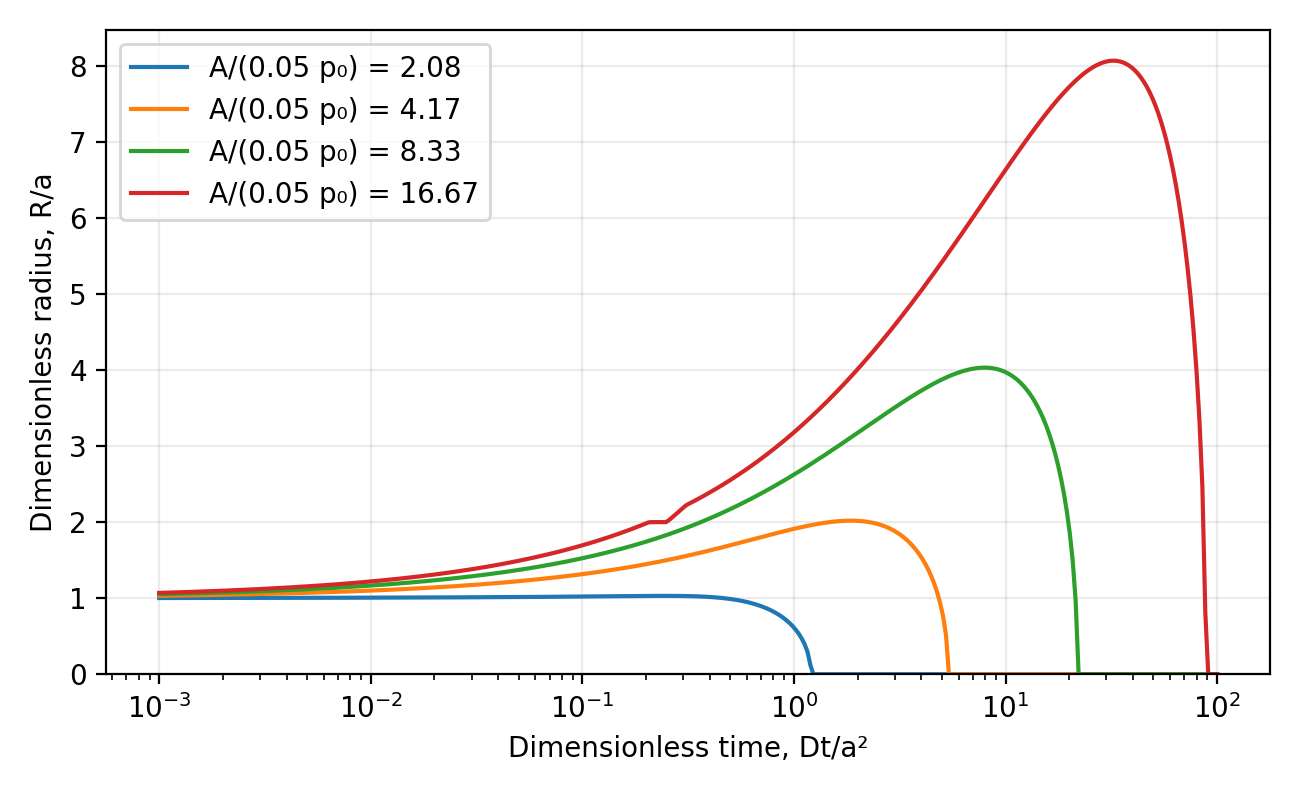
\includegraphics[width=0.62\textwidth]{p2_master}
\caption{Pressure-based stimulation radius under shut-in for several injection
strengths.}
\label{fig:p2_master}
\end{figure}

\subsection{Which Groups Matter, and Why the Soak-Time Sign Is Ambiguous}

The sensitivity of $R(t_s)$ is controlled mainly by $\Gamma$ and $P$.
Stress sensitivity changes the effective diffusivity during injection and
production, while $P$ sets the initial amplitude and therefore the
$\mathcal A$ that decides expansion versus contraction. $C_\phi$ and $\Lambda$
are secondary; $\Delta_d$ is inactive in the nominal range because the
compressive strain is below the damage threshold. The adsorption group $K_a$
does not affect the pressure radius, but it controls the nano front and
therefore the material-based radius.

This separation explains an apparent contradiction in the literature. Studies
that fix the total operation window report a weak negative correlation between
soak time and cumulative oil, because a longer soak consumes production time
\cite{p1-03}. In the present problem the production period is fixed at 360~d
after soaking; a longer soak does not consume production time, and its benefit
saturates as the material fronts slow down. The sign of the soak-time effect is
thus a property of the chosen time budget, not a universal physical law.

The four radius definitions of the problem statement differ by one to two
orders of magnitude. The pressure disturbance reaches tens of metres but
decays within days; the CO$_2$ and nano fronts move at sub-metre to metre
scales but persist; the damage radius is confined to the near-fracture zone.
For the Case~3 baseline the nano radius at 0.01~wt\% is about $0.15$~m with
the tabulated $K_d$ in m$^3$/kg, and about $0.52$~m if $K_d$ is interpreted
in L/kg; both values are grid-dependent and are reported with their mesh
refinement. The pressure radius is therefore not the limiting factor for a
long soak: the material fronts and the economics are.

% 05_p3_optimization.tex —— P3 多目标优化（你负责；T38 初稿 11/23 晚）
\section{Problem 3: Multi-Objective Optimization}

\subsection{Formulation}
[TBD: 目标 $Q_o$ 与 $C_{total}$（或 $\Delta NPV$）双目标；
设计变量 $C_n, q_{inj}, V_{inj}, f_{CO_2}, t_s, \tau_{inj}$ 及取值范围；
约束：设备能力、纳米 30 t/井次、$p_{max}=\min(0.95p_f, 60\ \mathrm{MPa})$、
$t_{inj}+t_s \le 90$ d；三情景 Case1/2/3。引 P3-02（技术+经济双维度合理性）。]

\subsection{Surrogate-Assisted Evaluation}
[TBD: LHS 500 点×3 情景批量正演；Kriging/RBF/RF 代理对比（10 折 CV，
$R^2>0.95$）；代理必要性引 P3-03；Pareto 回代真实正演校验误差 <10\%。]

\subsection{NSGA-II and Compromise Solutions}
[TBD: 种群 100、代数 200；每情景 2--3 个折中解（ knee 点选取准则写清楚）；
三情景可行域差异：Case1 空（工程不可行要如实报告）、Case2 上限约 137 m$^3$/d、
Case3 全区间。前沿图 + 折中解表。]

\subsection{Robustness Screening}
[TBD: 对渗透率、地应力等 ±15\% 扰动（说明分布与样本数，500 次）；
四项指标：工程可行率、$\Pr(\Delta NPV>0)$、最差 10\% 平均 $\Delta NPV$、均值±标准差；
$\mu-\sigma$ 为主判据，CVaR$_{0.9}$ 对照（引 P3-04）；工程建议。]

\subsection{Injection Timing and Fracture Closure}
[TBD（对应 T23，可并入 P1/P3）：$\tau_{inj}$ 等待期内缝宽
$w_f=w_{f,\infty}+(w_{f0}-w_{f,\infty})e^{-c_c(\sigma'_n-\sigma'_{n0})}$、
$k_f=w_f^2/12$、导流 $\propto w_f^3$（引 P1-07/P1-11）；
$\tau_{inj}$ 增大时 $w_f, k_f, NPV$ 单调下降；与折现影响分离。]

% 06_p4_data_econ.tex —— P4 数据模型与经济评价（队友；2026-11-20 定稿，
% 含 B1 反事实与增量 NPV）
\section{Problem 4: Data-Driven Production Model and Economic Evaluation}

\subsection{Data Partitioning and Quality Control}
The synthetic production data set (Attachment C) contains 38,880 records:
3 scenarios $\times$ 3 nano-concentrations $\times$ 12 soak-time levels
$\times$ 360 production days, with no missing values and no duplicated rows.
Daily oil rates carry $\pm5\%$ Gaussian noise with non-negative truncation;
truncated (zero) rates occur only in 36 of 108 groups, all in Case~1
(low-permeability) at late production times, and depress $Q_{360}$ by less
than 1--2\%. The bottom-hole pressure decays smoothly from an early maximum
(59.6 MPa in Case~3, briefly above the initial reservoir pressure as the
problem statement allows) and correlates with the oil rate ($\rho = 0.96$),
confirming physical consistency.

Following the blocked cross-validation principle \cite{p4-01}, we partition
by entire (case, $C_n$, $t_s$) groups rather than by individual days:
8 soak levels $\{5,10,20,25,30,35,40,50\}$ d form the training set (72 groups),
$t_s = 55$ d is the validation set, and $t_s \in \{15,45\}$ d (interpolation
hold-out) together with $t_s = 60$ d (extrapolation) form the test set.
The three subsets have no group overlap, and the test set contains soak levels
never seen in training, as required.

\subsection{Production Prediction Models}
We compare four regression models for the group-level cumulative oil
$Q_{360}$: a quadratic response surface, gradient boosting (depth-limited to
3 against over-fitting), random forest, and Gaussian-process (GP) regression
with an RBF kernel; features are $C_n$, $t_s$, their interaction $C_n t_s$,
$\log t_s$, and scenario indicators (the feature set fixed a priori before
any test evaluation). Model selection uses GroupKFold with entire soak levels held
out (8 folds), mirroring the extrapolation task. The GP achieves the best
cross-validated RMSE (25.1 m$^3$ mean, 82.0 worst fold; MAPE 4.6\%) and
validation MAPE of 1.6\%; the tree
ensembles cannot interpolate a withheld interior soak level (their
predictions are piecewise constant in $t_s$), which disqualifies them for the
soak-time scan despite good endpoint behavior. The quadratic surface
under-fits the saturation trend. Simple baselines confirm the need for
nonlinearity: a constant predictor attains 13\% MAPE, a plain linear model
74\%, and a log-$t_s$ linear model 27\%.

The GP is frozen (features and hyper-parameter grid fixed) and evaluated on
the test set exactly once (Table~\ref{tbl:p4_test}): MAPE is 0.53\% on the
interpolation hold-out and 3.59\% on the $t_s = 60$ d extrapolation, well
within the 15\% target, with rank correlation above 0.98 everywhere.

\begin{table}[h!t]
\centering
\caption{Frozen GP: one-shot test performance for $Q_{360}$.}
\label{tbl:p4_test}
\small
\begin{tabular}{lccccc}
\toprule[1.5pt]
Subset & $n$ & RMSE (m$^3$) & MAPE (\%) & Spearman\\
\midrule[1pt]
Interpolation ($t_s=15/45$) & 18 & 11.6 & 0.53 & 1.000\\
Extrapolation ($t_s=60$)    & 9  & 26.6 & 3.59 & 0.983\\
\bottomrule[1.5pt]
\end{tabular}
\end{table}

Prediction uncertainty is quantified with the GP posterior std. Out-of-fold
95\% intervals cover 94.4\% of training groups (nominal 95\%), so the raw
posterior is close to calibrated; a variance-scaling calibration
($\kappa = 0.47$) degrades coverage to 80.6\% and is therefore not adopted.
On the test set the coverage is 92.6\%, reflecting honestly widened
intervals under extrapolation. Interpretability analysis (permutation
importance and partial-dependence
plots) attributes 74\% of predictive power to the scenario indicators
(permeability contrast between cases), 20\% to the soak time, and only
6\% to the nano-concentration within the studied range; the partial-dependence
curves show $Q_{360}$ increasing near-linearly in $C_n$ and saturating in
$t_s$, consistent with the $\sqrt{t}$ pressure-diffusion scaling of the
mechanistic model (Section~4).

\subsection{Economic Evaluation under Appendix B}
The economic module strictly follows Appendix~B: all volumes are metered at
the 25 MPa, 300 K reference state; $t_{inj} = V_{inj}/q_{inj}$; cash flows
are discounted daily at $r = 8\%$/yr from day 0; the injection fee accrues
over the actual injection days, the soak fee over $t_s$, and the production
phase carries only variable costs ($c_{prod} = 0.035$, $c_{water} = 0.0025$
10$^4$ CNY/m$^3$). The implementation reproduces the worked example of the
problem statement to the cent (848.25$\times10^4$ CNY for
$V_{inj}=3000$ m$^3$, $f_{CO_2}=0.5$, $C_n=1.0$ wt\%, 10 d injection and
30 d soak). Produced-water data are absent from Attachment~C (a known data
gap); we adopt a water--oil ratio $WOR = 0.5$ and show that NPV varies by
less than 2\% over $WOR \in [0,2]$.

Figure~\ref{fig:p4_npv} shows NPV versus soak time for the three scenarios
at the baseline operation ($q_{inj}=300$ m$^3$/d, $V_{inj}=3000$ m$^3$,
$f_{CO_2}=0.5$, $\tau_{inj}=0$). The economically optimal soak time
(maximizing NPV) is $t_s^* = 10$ d for Case~1, 20--25 d for Case~2, and
30--40 d for Case~3 (35 d at $C_n=1.0$). Only Case~3 attains a positive
absolute NPV (up to $+284\times10^4$ CNY at $C_n=0.5$, $t_s=40$ d);
Case~1 and Case~2 remain negative at all soak levels because the 3000 m$^3$
fluid slug dwarfs the producible volume---a conclusion independently
supported by the injectivity analysis of the mechanistic model, which shows
Case~1 cannot even accept 300 m$^3$/d without exceeding $p_{max}$
(Section~5). Breakeven oil prices at $t_s^*$ are 796 USD/bbl (Case~1),
157 USD/bbl (Case~2) and 64 USD/bbl (Case~3, below the 75 USD/bbl market
price), i.e.\ Case~3 is the only economically viable scenario under the
baseline operation. Following the requirement to report loss categories
separately, we distinguish (i) engineering infeasibility (violation of
$p_{max}$, handled as a hard constraint in Section~5), (ii) absolute
NPV $<0$ (all 36 Case~1 and Case~2 combinations tested, 6 of 36 in
Case~3), and (iii) $\Delta NPV = NPV - NPV_{B1}$ against the
fracturing-only baseline $B1$.

\paragraph{Fracturing-only counterfactual.}
For $B1$, production starts from the initial pressure and saturations,
with no injection or soak. We retain the fracture geometry, well-pressure
and liquid limits, and use the tank decline with the case-specific
storage length from the $C_n=1.0$~wt\%, $t_s=30$~d training fit.
The same $WOR=0.5$ is used. Over 360~d, only the initial fracturing
cost and variable production and water costs are charged.
For Cases~1--3, respectively, $NPV_{B1}$ is $-33.58$, $280.47$ and $915.97$
in units of $10^4$~CNY. At each case's best reference-operation combination
(all at $C_n=0.5$~wt\%), $\Delta NPV$ is $-539.55$, $-595.40$ and $-632.45$
in the same units. Case~3 has positive absolute NPV and negative
incremental NPV under this storage-length assumption. Attachment~C
contains no fracturing-only production series, so these incremental
values depend on the counterfactual storage model. In Case~3 the incremental NPV changes sign at a B1 storage length of about 0.176~m under the same rate and cost assumptions \cite{codex}.

\subsection{Mechanism--Data Comparison}
Figure~\ref{fig:p4_overlay} overlays the frozen-GP $Q_{360}(t_s)$ curves
on the observed group means at $C_n = 1.0$ wt\%. Two viewpoints on the
optimal soak time emerge, as anticipated in the master plan. The
\emph{production} viewpoint defines $t_s^*$ as the inflection point of the
cumulative-production-increment curve \cite{p4-04}, which the GP curves
place at the earliest scanned level (5~d) in all three scenarios---the
increment decays monotonically from the start. The \emph{economic}
viewpoint of \S6.3 instead yields interior optima (10/20/35~d at $C_n=1$~wt\%), because
daily discounting and the soak-day fee shift the optimum to shorter
soaks; the two definitions are both reported and their divergence is
explained by the time-budget difference, not by physics
\cite{p4-04, p4-05}.

Three effects limit the mechanism--data comparison.
\emph{Model assumptions:} the tank model uses a fixed calibrated storage
length in its independent Case~3 check. Its cumulative error is 5.36\% at
55~d, and it misses the observed gain from 30 to 55~d. Local damage tests
at prescribed pressure histories yield $d=0$ at the nominal thresholds.
\emph{Numerical error:} at the 0.01~wt\% threshold the calculated nano
radius changes from zero with 50 cells to 0.15~m with 200 cells in the
Case~3 injection test. The radius remains grid-dependent.
\emph{Data noise:} Attachment~C contains synthetic daily variability.
The within-group rate CV also includes the production decline, so the
decline and noise are treated separately when interpreting the residuals.
Figure~\ref{fig:p4_overlay} compares the frozen data model with Attachment~C.

\begin{figure}[h!t]
\centering
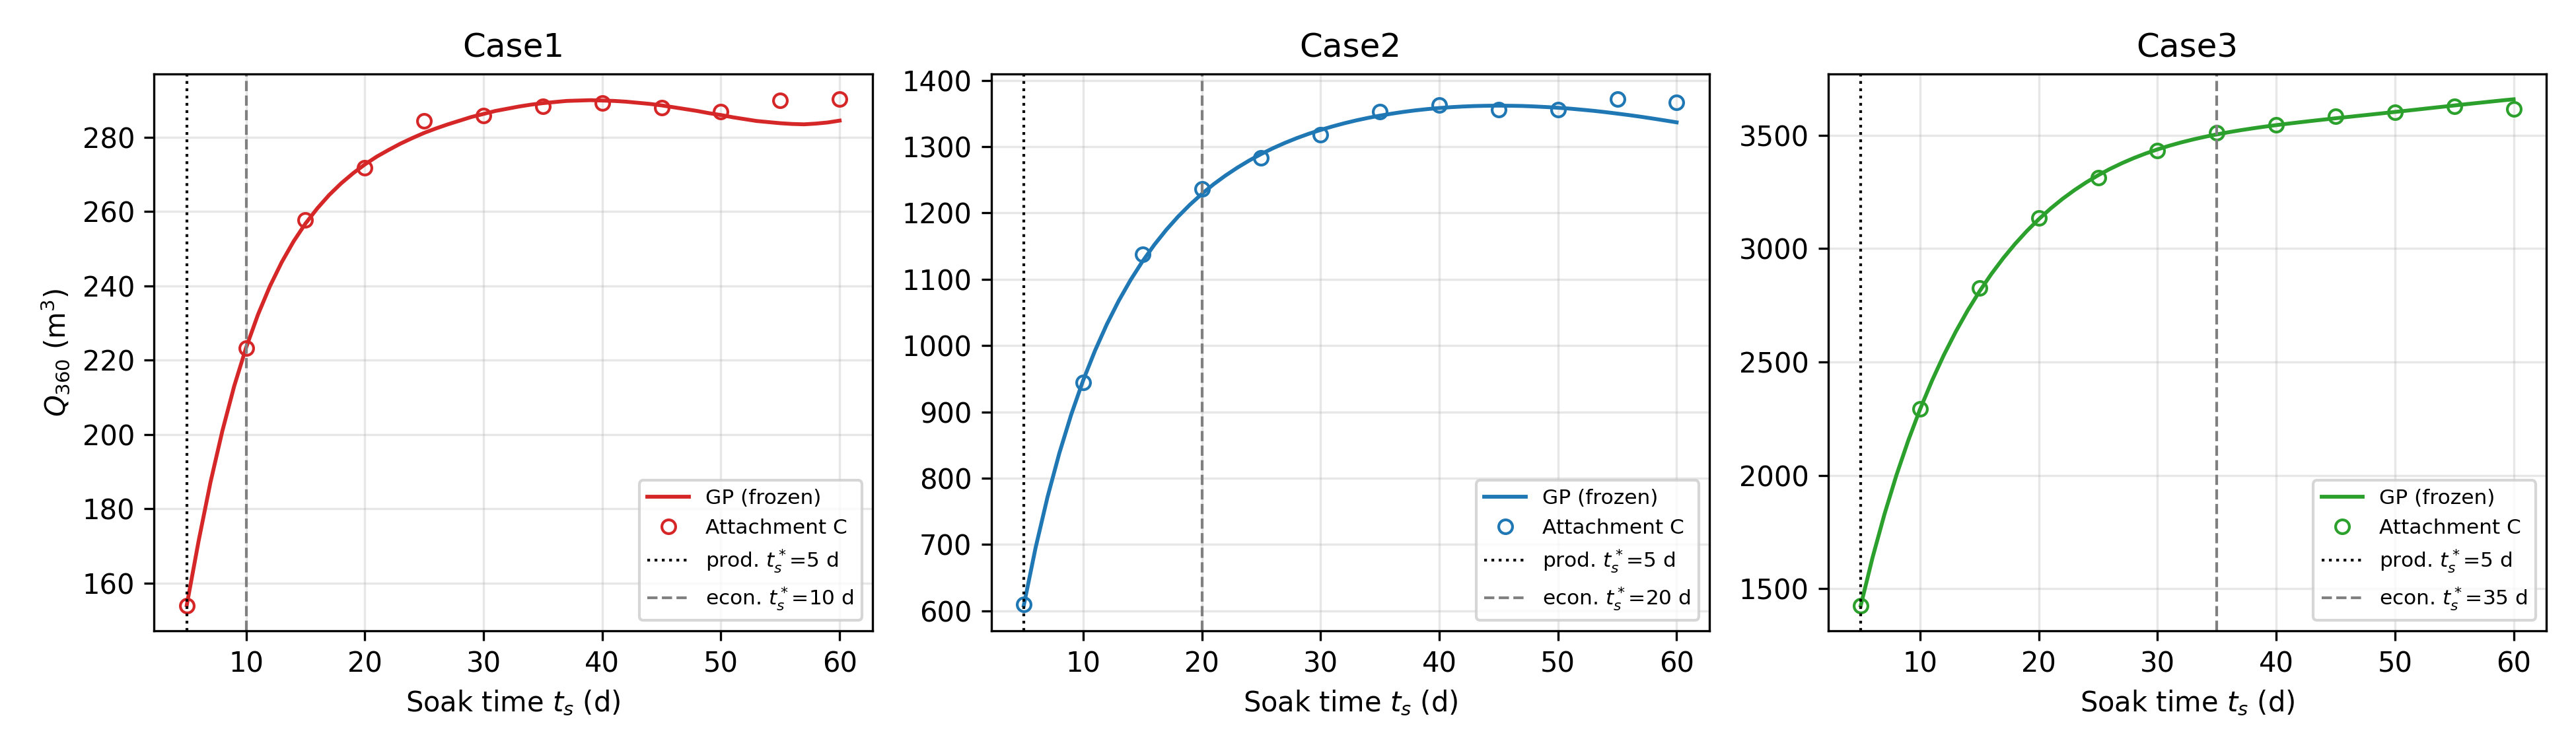
\includegraphics[width=\textwidth]{p4_mech_data.png}
\caption{Frozen-GP production curves $Q_{360}(t_s)$ (lines) versus
observed group means (circles) at $C_n = 1.0$ wt\%; economic-optimum
soak levels (ticks) are interior while production-increment inflection
occurs at the earliest level.}
\label{fig:p4_overlay}
\end{figure}

% 图表（T36/T37 定稿统一编号）：
%   fig:p4_split   T03_split_overview.png      数据划分
%   fig:p4_models  T12_model_comparison.png    模型对比 + val 散点
%   fig:p4_npv     T16_npv_ts_curves.png       NPV–ts 曲线
%   fig:p4_interpret T15_interpretability.png  重要性 + PDP

\begin{figure}[h!t]
\centering
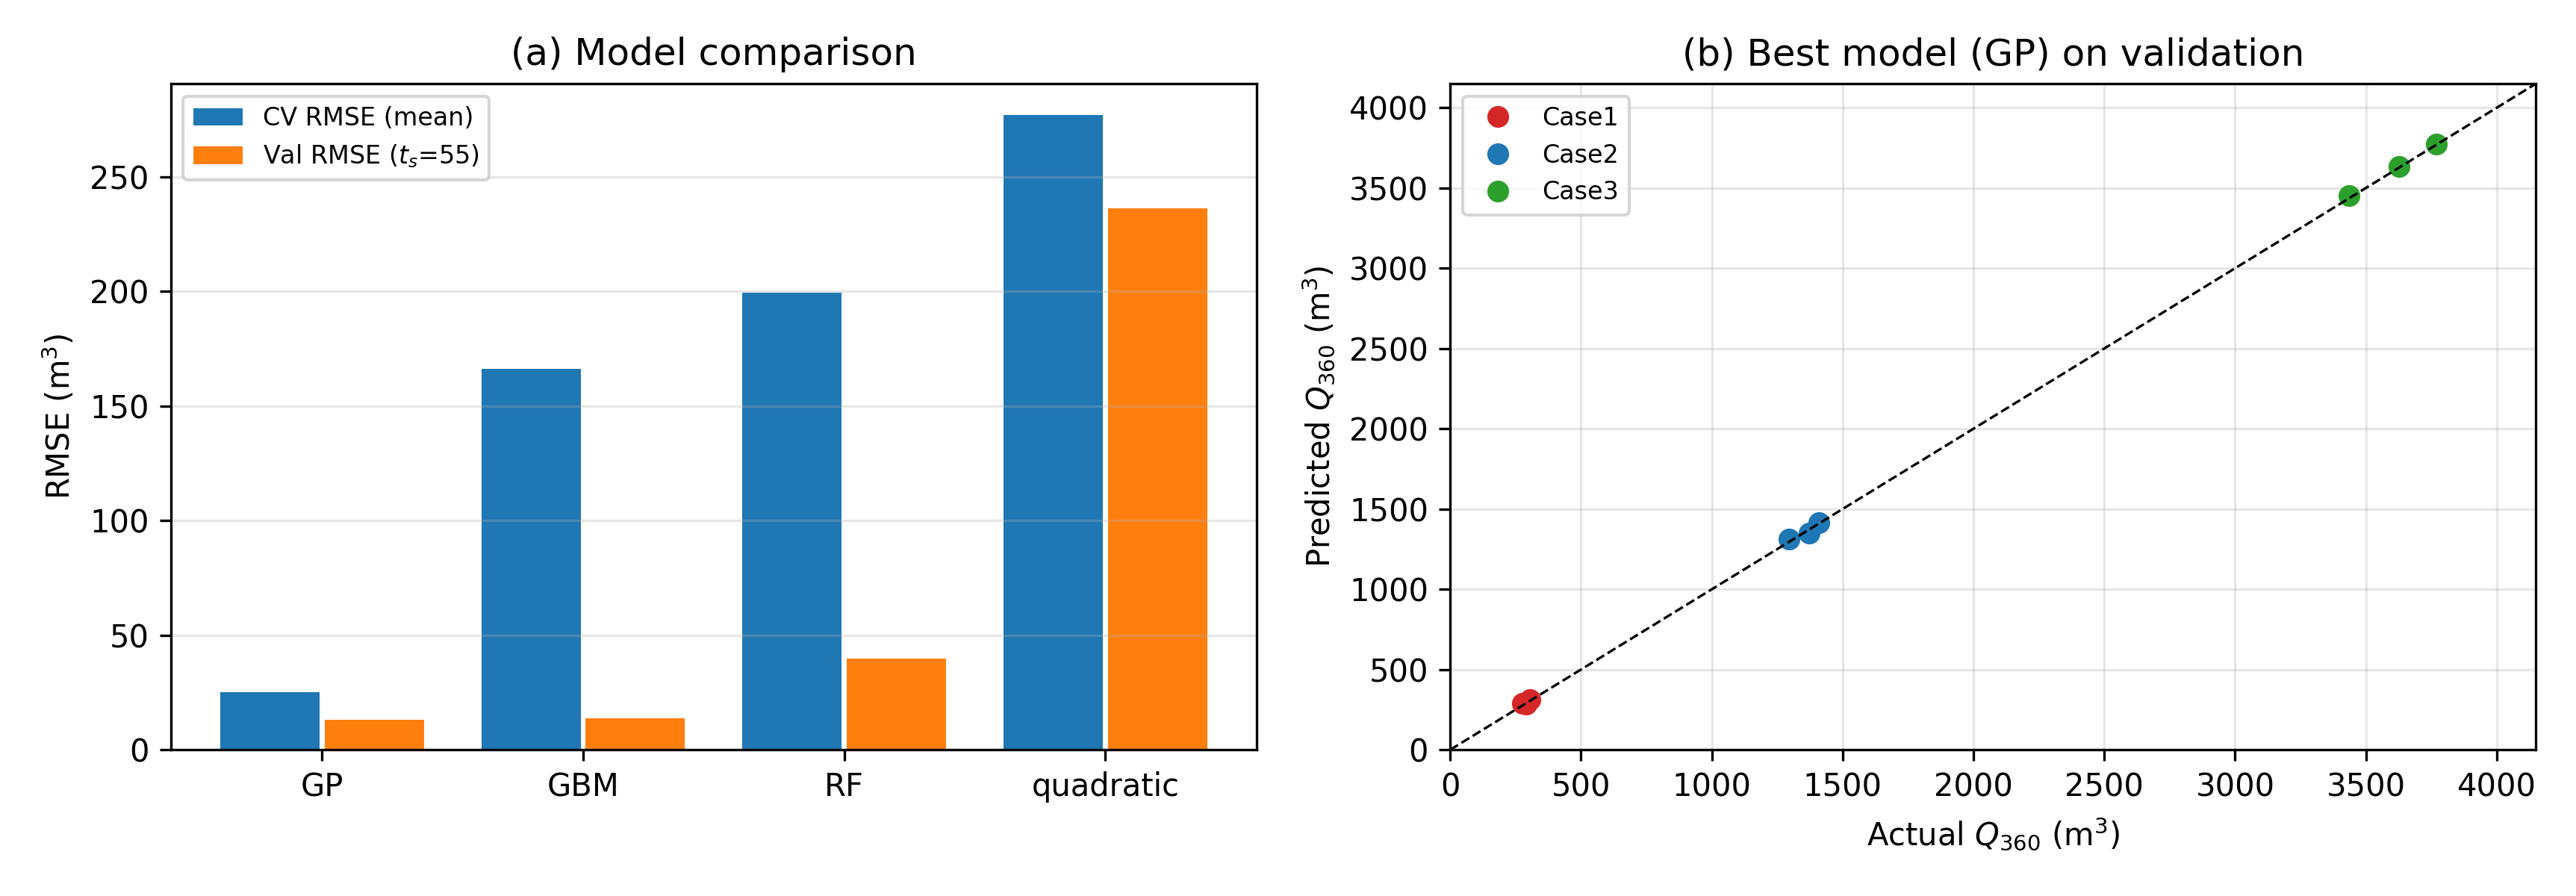
\includegraphics[width=0.9\textwidth]{p4_model_comp.png}
\caption{Model comparison for $Q_{360}$ (GroupKFold by soak level): the
GP dominates; tree ensembles fail to interpolate withheld interior soak
levels; baselines confirm the need for nonlinear features.}
\label{fig:p4_models}
\end{figure}

\begin{figure}[h!t]
\centering
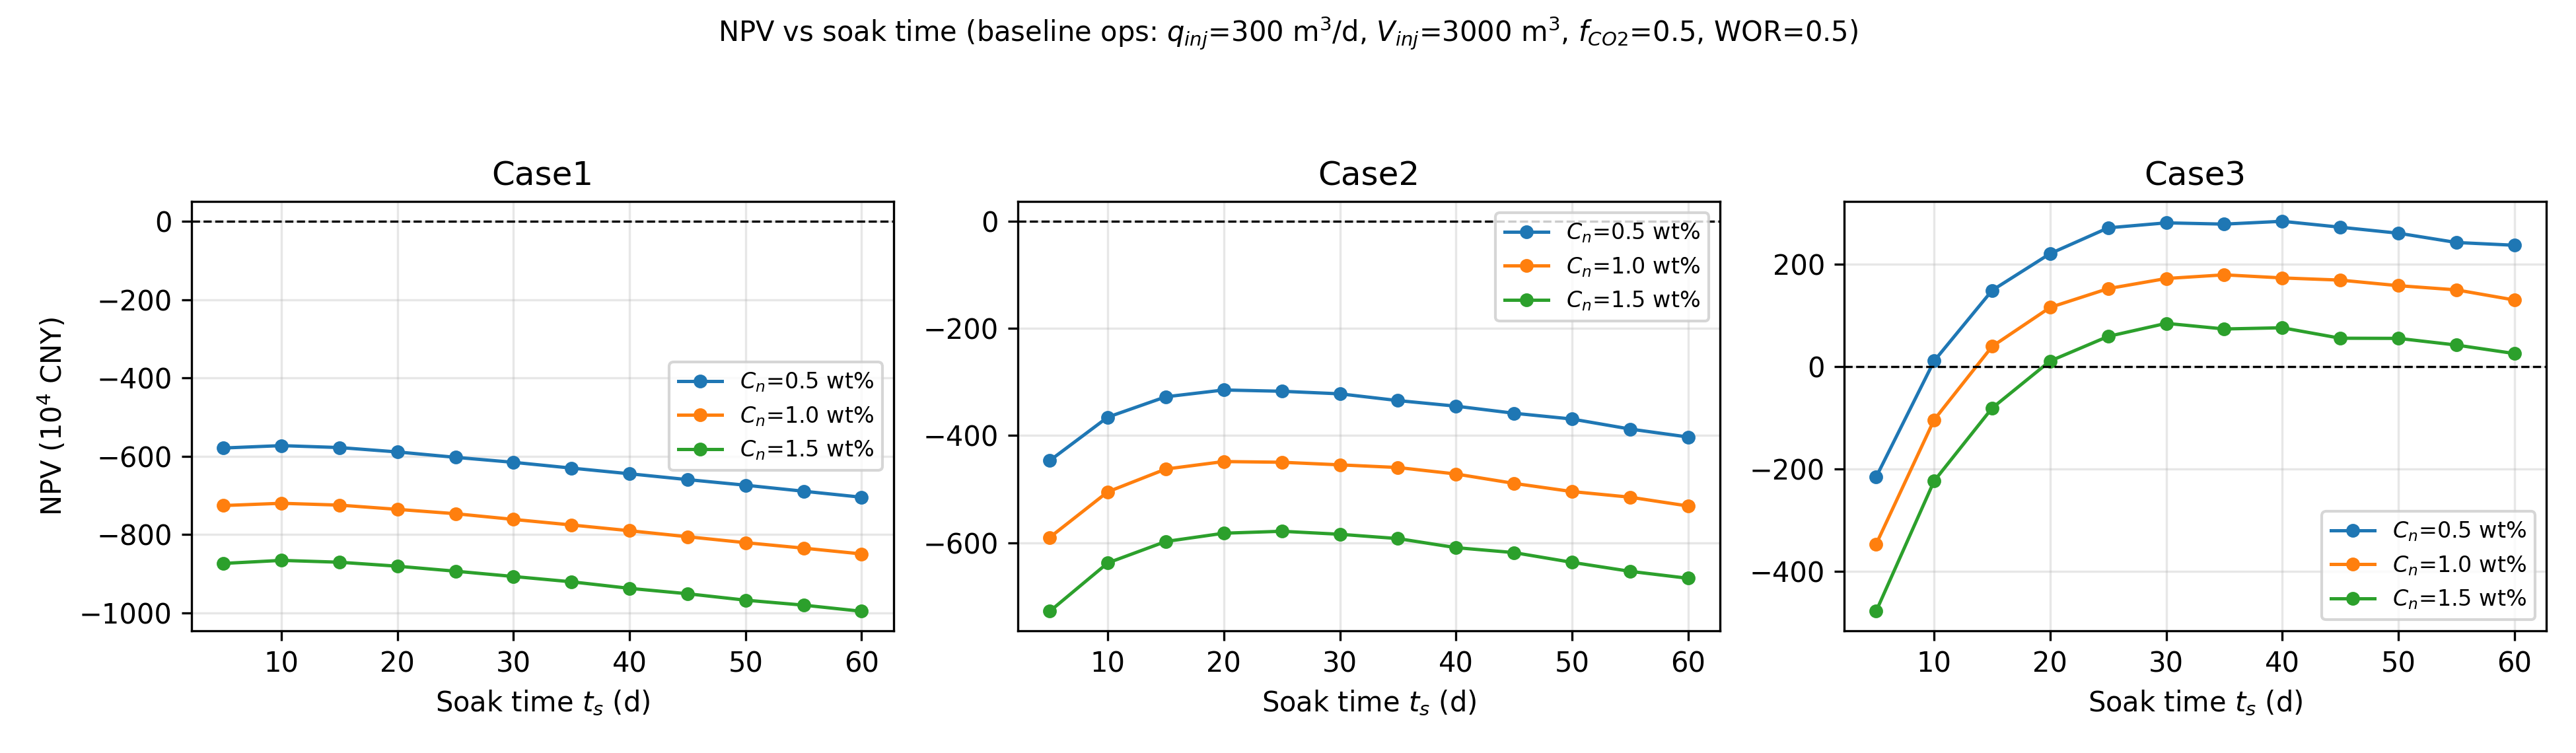
\includegraphics[width=0.9\textwidth]{p4_npv_ts.png}
\caption{NPV versus soak time at baseline operation; interior economic
optima in all scenarios, positive NPV only in Case~3.}
\label{fig:p4_npv}
\end{figure}

\begin{figure}[h!t]
\centering
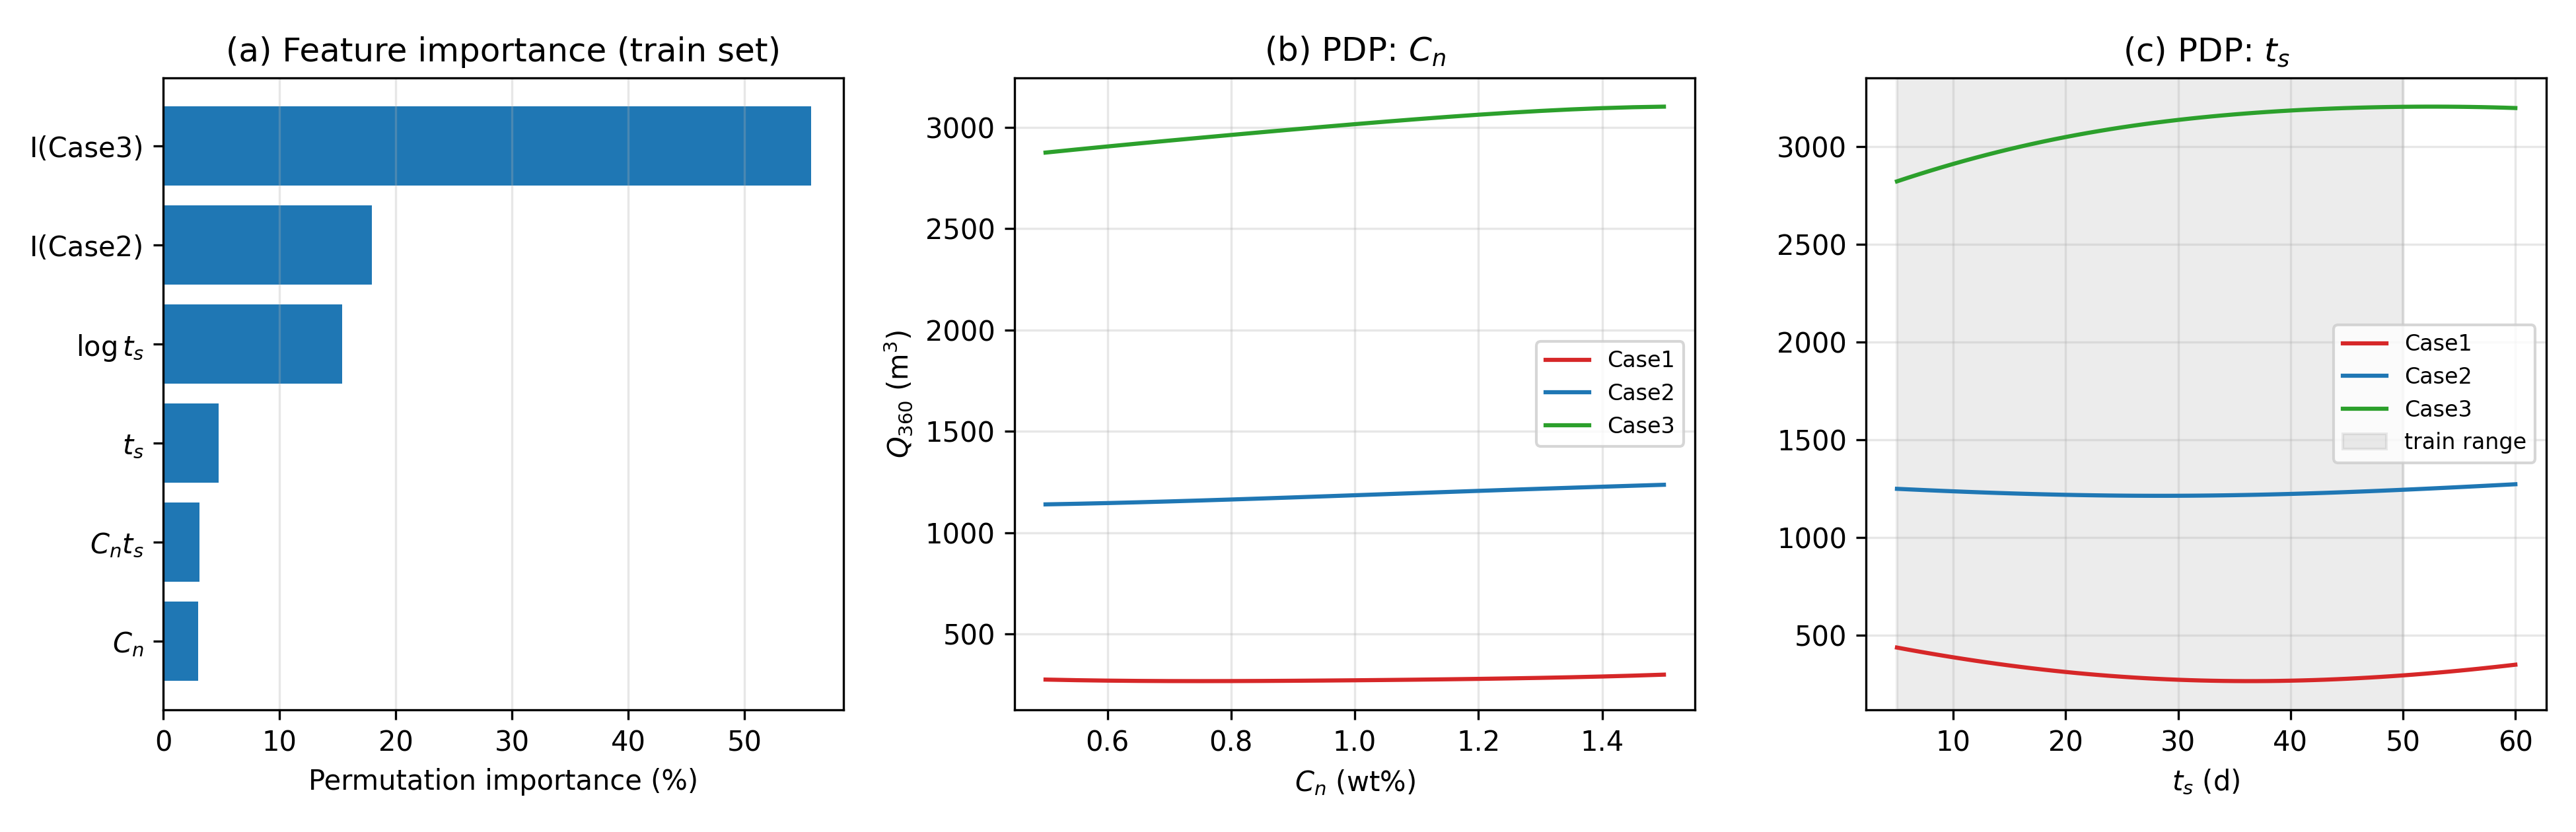
\includegraphics[width=0.9\textwidth]{p4_importance.png}
\caption{Permutation importance and partial-dependence profiles of the
frozen GP; scenario identity dominates, $C_n$ contributes least.}
\label{fig:p4_interpret}
\end{figure}

% 07_evaluation_sensitivity.tex —— 综合评价指标体系 + Sobol 全局敏感性（队友）
\section{Comprehensive Evaluation and Global Sensitivity}

\subsection{Evaluation Indicator System}
To rank stimulation strategies beyond a single objective, we define seven
indicators, each with a clear unit and direction (Table~\ref{tbl:indicators}).
Indicators are min--max normalized so that larger is always better, and the
radar chart (Figure~\ref{fig:radar}) compares the three scenarios at their
economically optimal soak time. Case~3 dominates all axes; Case~2 shows
decent productivity but weak economics; Case~1 trails everywhere, consistent
with the economic analysis of Section~6. The stimulation radius $R(t_s^*)$
(from Section~4) and the robustness margin (from Section~5) plug into the
same framework as additional axes.

% 数值表定稿时从 03_结果与图表/T26_indicator_table.csv 誊入
\begin{table}[h!t]
\centering
\caption{Comprehensive evaluation indicators (larger is better after
normalization; evaluated at each scenario's economic optimum, $C_n=1.0$ wt\%).}
\label{tbl:indicators}
\small
\begin{tabular}{clccc}
\toprule[1.5pt]
No. & Indicator (unit) & Case1 & Case2 & Case3\\
\midrule[1pt]
I1 & $Q_{360}$ (m$^3$)                  & 223   & 1236  & 3512\\
I2 & NPV ($10^4$ CNY)                  & $-721$ & $-449$ & 179\\
I3 & Unit cost (10$^4$ CNY/m$^3$)      & 3.57  & 0.70  & 0.28\\
I4 & Soak gain $Q_{360}(t_s^*)/Q_{360}(5\,\mathrm{d})$ (-)
                                       & 1.45  & 2.03  & 2.46\\
I5 & Nano marginal gain (m$^3$/wt\%)  & 21    & 108   & 320\\
I6 & Breakeven margin $P^*/P_{be}$ (-) & 0.09  & 0.48  & 1.18\\
I7 & Test MAPE (\%)                    & 3.27  & 0.87  & 0.51\\
\bottomrule[1.5pt]
\end{tabular}
\end{table}

\subsection{Nested Sobol Sensitivity Analysis}
[TBD T35: Saltelli sampling ($N = 1024$); outer loop samples all key
geological/engineering parameters except $t_s$; for each outer sample the
inner loop scans $t_s$ and records the NPV-maximizing $t_s^*$; report the
total-effect Sobol indices of $Q_{360}$ and $t_s^*$, identify the top-3
parameters controlling $t_s^*$, and compare the ranking with the reference
study \cite{p4-04} (injected volume $>$ capillary-pressure multiplier
$>$ matrix permeability $>$ $\dots$). Consistency corroborates the
mechanistic model; deviations are explained by the additional nano and
CO$_2$ variables in our design. Methodology follows \cite{p4-02}.]

% 图表：fig:radar → T26_radar.png（T37 统一编号定稿）

% 08_conclusion.tex —— 优缺点与结论
\section{Strengths and Weaknesses}

The main strength is consistency. Problems~1--4 share one symbol set, one
forward model and one economic convention. The pressure redistribution of
Problem~2 is validated against the three-phase simulation of Problem~1; the
reduced production model of Problem~3 is calibrated to the training groups of
Problem~4; and the economic evaluation follows Appendix~B exactly, including
the reference state, the daily discounting and the fracturing-only baseline.
The robustness metrics are separated into feasibility, conditional
profitability and joint frequency, which keeps an infeasible candidate from
being reported as merely uneconomic.

The limitations are equally explicit. The model is one-dimensional normal to
the fracture, so pressure loss along the fracture and lateral interference are
neglected. Natural fractures in Case~3 are represented by an equivalent
permeability rather than a dual-porosity model. Water production is not
supplied, so the produced-water term uses a constant water--oil ratio. The
damage variable is inactive in the nominal pressure range, and the effect of
injected volume and CO$_2$ fraction on production is not identifiable from the
supplied data; the zero-exponent convention and the positive-exponent control
are both reported.

\section{Conclusion}

For Problem~1, the single-phase benchmark shows approximately second-order
spatial and first-order temporal convergence. Table~\ref{tbl:verification}
gives mass-balance errors for the tested flow settings. For Problem~2, the
Case~3 numerical 5\% pressure radius vanishes between 3 and 4~d at
300~m$^3$/d and between 6 and 8~d at 800~m$^3$/d. Both analytical
comparisons give earlier loss of the threshold in these tests.

For Problem~3, Case~1 has no feasible point in the prescreen. Three low-rate
three-phase runs exceed the pressure limit before the planned volume is injected. Case~2 is
feasible but uneconomic: the compromise candidates give NPV between $-164$
and $-87\times10^4$~CNY, with a joint feasibility--profitability frequency of
zero. Case~3 is the only robustly viable scenario: NPV ranges from $+365$ to
$+671\times10^4$~CNY, all 200 samples per candidate pass the reduced prescreen and have positive NPV. The compromise soak times are $8$--$24$~d under the calibrated
production model.

The engineering implications are conditional. Further pressure tests would be needed to establish a viable injection window
for Case~1. Case~2 remains uneconomic for the three selected candidates at
the baseline oil price. Case~3 supports the
lowest-cost operating point under the zero-exponent convention; if a positive
volume or CO$_2$-fraction benefit is later demonstrated, the preferred injected
volume moves from $1000$ to about $1668$~m$^3$. The absolute NPV values should
be read together with the uncalibrated water-production and baseline terms.


%----------------------------参考文献
% 09_references.tex —— 参考文献（统稿维护）
% 书目信息按 05_文献/文献映射.md 预填；标注 [check] 的字段定稿前从 PDF 首页核对
\begin{thebibliography}{29}

\bibitem{p1-03} Xia et al., Design of CO$_2$ huff-n-puff parameters for fractured tight oil reservoirs considering geomechanical effects. \emph{Processes}, 2024. %[check]
\bibitem{p1-04} Rezk and Foroozesh, Phase behavior and fluid interactions of a CO$_2$--light oil system at HPHT conditions. %[check]
\bibitem{p1-05} Li et al., The impact of nanoparticle adsorption on transport and wettability alteration. \emph{Frontiers in Physics}, 2019. %[check]
\bibitem{p1-06} Zhang et al., Quantitative investigation of nanofluid imbibition in tight oil reservoirs based on NMR. 2022. %[check]
\bibitem{p1-07} Wang and Sharma, Estimating unpropped fracture conductivity and fracture compliance from DFIT. %[check]
\bibitem{p1-08} Rostami et al., Shape factor for regular and irregular matrix blocks in fractured porous media. \emph{Petroleum Science}, 2019. %[check]
\bibitem{p1-09} Lee, Wheeler and Wick, Iterative coupling of flow, geomechanics and adaptive phase-field fracture. %[check]
\bibitem{p1-10} Hamiel, Lyakhovsky and Agnon, Poroelastic damage rheology. \emph{Geochemistry, Geophysics, Geosystems}, 2005. %[check]
\bibitem{p1-11} Jia, Ma, Cheng and Clarkson, Semi-analytical model for hydraulic fractures during flowback. \emph{Energy Science \& Engineering}, 2020. %[check]
\bibitem{p1-12} Hamiel, Lyakhovsky and Agnon, Coupled evolution of damage and porosity. \emph{Geophysical Journal International}, 2004. %[check]
\bibitem{p1-13} Zhang, Hu and Zhang, CO$_2$ huff-n-puff considering molecular diffusion and adsorption. \emph{Energies}, 2019. %[check]
\bibitem{p1-14} Merxhani, An introduction to linear poroelasticity. 2016. %[check]
\bibitem{p1-15} Nasser et al., Hybrid nanofluid wettability alteration and fracturing for CO$_2$ huff-n-puff. \emph{Energy Geoscience}, 2026. %[check]

\bibitem{p2-01} Rice and Cleary, Some basic stress diffusion solutions for fluid-saturated elastic porous media. \emph{Reviews of Geophysics}, 1976. %[check]
\bibitem{p2-02} Mahzari et al., Novel laboratory investigation of huff-n-puff gas injection for shale oils. %[check]
\bibitem{p2-03} Schmid and Geiger, Universal scaling of spontaneous imbibition. \emph{Water Resources Research}, 2012. %[check]
\bibitem{p2-04} Zhang et al., CO$_2$ huff-and-puff in tight sandstone: NMR study. %[check]
\bibitem{p2-05} Alotaibi et al., Stream and potential functions for transient flow. \emph{Fluids}, 2023. %[check]
\bibitem{p2-06} Fakcharoenphol et al., Effect of shut-in time on gas flow rate in hydraulically fractured shale reservoirs. \emph{Journal of Natural Gas Science and Engineering}, 2016. %[check]

\bibitem{p3-01} Wang et al., Optimization and analysis of CO$_2$ huff-n-puff using response surface methodology. \emph{Geofluids}, 2022. %[check]
\bibitem{p3-02} Zhang Jie et al., Sensitivity analysis and multiobjective optimization of CO$_2$ huff-n-puff. 2021. %[check]
\bibitem{p3-03} Kim and Durlofsky, A CNN--RNN proxy for robust optimization. %[check]
\bibitem{p3-04} Capolei et al., Risk minimization in life-cycle oil production optimization. %[check]
\bibitem{p3-05} Khanal and Shahriar, Optimization of CO$_2$ huff-n-puff in unconventional reservoirs. \emph{Energies}, 2023. %[check]

\bibitem{p4-01} Roberts et al., Cross-validation strategies for data with temporal, spatial, hierarchical, or phylogenetic structure. \emph{Ecography}, 2017. %[check]
\bibitem{p4-02} Saltelli et al., Variance based sensitivity analysis of model output: total sensitivity index. \emph{Computer Physics Communications}, 2010. %[check]
\bibitem{p4-04} Wang Qiang et al., Optimization method of post-fracturing soak time for shale oil reservoirs. \emph{Petroleum Exploration and Development}, 2022. %(in Chinese) %[check]
\bibitem{p4-05} Yang and Fang, Economic feasibility evaluation of CO$_2$ huff-and-puff. 2026. %[check]

\end{thebibliography}

\label{LastMainPage}

\clearpage
\pagestyle{plain}
\section*{AI Tool Use Report}
\phantomsection
\addcontentsline{toc}{section}{AI Tool Use Report}

This disclosure follows the contest AI-use rules. Both tools were used on
20 November 2026, as evidenced by the project exchanges of that date. Only
content confirmed by the team is recorded below.

\paragraph{DeepSeek (DeepSeek AI; model variant unconfirmed).}
Documented use: 20 November 2026. At that date the vendor's production API
served the V4 family (public release record: V4 preview, 24 April 2026;
V4-Pro general availability, 13 August 2026; V4.1-Flash, 10 September
2026); the exact variant answering the team's queries is not recorded.
Representative requests: implement and check the P1--P4 simulation chain;
write calibration, data-analysis and optimization code; fit the
production surrogate to the training groups and rerun the optimization
with the calibrated volume and composition responses. Adopted content: the
corresponding scripts and selected result files in the supporting
archive, together with generated plots and numerical outputs for pressure
redistribution, damage, production calibration and the optimization
runs. The modeling and programming teammates checked the key assumptions,
formulas and scripts before adoption.

\paragraph{Codex (OpenAI; GPT-6 family; exact variant unconfirmed).}
Documented use: 20 November 2026. Public release record of the family:
GPT-6 Astra, 3 September 2026; GPT-6 Sol and Luna, 22 September 2026;
GPT-6.1 Sol, 29 September 2026 (default in Codex CLI from late September
2026). Representative requests: review and repair the implementation;
check the paper against the verification reports and contest
requirements; prepare the submission files; write the fracturing-only B1
comparison and the break-even storage-length calculation. Adopted content:
reviewed code, the B1 comparison and break-even calculation (the B1
values reported in the text are calculations from the reduced production
proxy), manuscript edits and reference corrections, and the compiled-PDF
and reproduction-package checks. The writing teammate rewrote the adopted
AI-generated text during final editing.

\paragraph{Human review and independent verification.}
The core modeling, solution strategy and conclusions were completed
independently by the team; AI outputs served as drafts and were checked
before adoption. Recorded checks include: (i) an independent
re-implementation of the Sobol sampling design and total-order estimator
(\texttt{sobol\_lib.py}), validated on the Ishigami test function and by
replication of the forward evaluation (agreement to $10^{-13}$);
(ii) rerunning the cross-validation after the feature set was aligned
with the model outline (CV RMSE 25.1; frozen-test MAPE 0.53\% and
3.59\%); (iii) verifying the economic self-check against the worked
example of the problem statement ($848.25\times10^4$~CNY reproduced
exactly) and reproducing the B1 incremental NPVs from the packaged
inputs; and (iv) checking every bibliography entry against the source
documents. The B1 baseline remains a fracturing-only model
counterfactual and still lacks independent production observations.


% ---------------------附录（推导、代码清单、补充图表）
\newpage
\pagestyle{plain}
\section*{Appendix}
\addcontentsline{toc}{section}{Appendix}
\subsection*{A.1 Mirror-kernel derivation}

The shut-in problem is
\begin{equation}
\frac{\partial u}{\partial t}=D\frac{\partial^2u}{\partial x^2},
\qquad x>0,\qquad
\left.\frac{\partial u}{\partial x}\right|_{x=0}=0,\qquad u\to0\ \ (x\to\infty).
\end{equation}
The zero-flux condition is enforced by the even extension of the initial
disturbance to $x<0$. For a step $u_0=A$ on $[0,a]$, integrating the Gaussian
kernel against the even extension gives Eq.~\eqref{eq:kernel}. The threshold
root in Eq.~\eqref{eq:threshold} is unique because $u(x,t_s)$ decreases
monotonically in $x$; it is found by bisection on a fine grid. When
$u(0,t_s)<0.05p_0$ the root does not exist and $R=0$ by definition. The
constant-pressure step result, Eq.~\eqref{eq:erfc}, follows from the
complementary error function with $\Theta=0.05p_0/(p_{inj}-p_0)$.

\subsection*{A.2 Dimensionless groups}

The groups in Table~\ref{tbl:pi_groups} are obtained by substituting the
scales of Eq.~\eqref{eq:scales} into the flow, transport, stress and damage
equations. The magnitudes use Case~3 parameters; Case~0 gives
$P=0.27$, $\Gamma=2.25$ and $C_\phi=0.027$. The adsorption group is evaluated
with the initial water saturation, $K_a=(1-\phi)\rho_rK_d/(\phi S_w)$.

\subsection*{A.3 Economic cash flow and self-check}

The total cost and the daily cash flow follow Appendix~B of the problem:
\begin{equation}
C_{total}=C_{frac}+c_{inj}t_{inj}+c_{soak}t_s+C_{nano}+C_{CO_2}
+c_{prod}Q_o+c_{water}Q_w,
\end{equation}
\begin{equation}
CF(t)=P_{oil}^*Q_o-c_{prod}Q_o-c_{water}Q_w
-c_{inj}I_{inj}-c_{soak}I_{soak}-c_{nano}m_{nano,day}-c_{CO_2}m_{CO_2,day},
\end{equation}
\begin{equation}
NPV=-C_{frac}+\sum_{t=1}^{T}\frac{CF(t)}{(1+r)^{t/365}},
\qquad T=t_{inj}+t_s+360 .
\end{equation}
The fracturing-only baseline $B1$ uses $T=360$~d.
Run \texttt{13\_b1\_comparison.py} to reproduce the incremental NPVs. The implementation
reproduces the worked example of the problem statement exactly:
$300+38.25+300+90+120=848.25\times10^4$~CNY for $V_{inj}=3000$~m$^3$,
$f_{CO_2}=0.5$, $C_n=1$~wt\%, $t_{inj}=10$~d and $t_s=30$~d.

\subsection*{A.4 Code and reproduction}

\begin{table}[h!t]
\centering
\caption{Main code modules.}
\small
\begin{tabular}{ll}
\toprule[1.5pt]
File & Purpose\\
\midrule[1pt]
\texttt{config.py} & parameter tables, SI conversion, reference state\\
\texttt{model/three\_phase.py} & three-phase flow, CO$_2$ and nano transport\\
\texttt{model/two\_phase.py} & oil--water baseline\\
\texttt{model/nano\_transport.py} & Langmuir adsorption and scalar transport\\
\texttt{model/p2\_scaling.py} & mirror kernel and $R(t_s)$\\
\texttt{model/production.py} & reduced production model\\
\texttt{model/p3\_forward.py} & P3 evaluator\\
\texttt{model/nsga2.py} & NSGA-II\\
\texttt{model/waiting.py} & fracture closure during waiting\\
\texttt{model/mechanics.py} & poroelastic strain and damage\\
\bottomrule[1.5pt]
\end{tabular}
\end{table}

Numbered scripts in the code directory write their validation results to the
results directory, which also holds the source figures.
Compile with \texttt{xelatex main.tex} twice to resolve cross-references.

\subsection*{A.5 Supplementary sensitivity}

The nano radius is grid-dependent: at 10~d and $C_n=1$~wt\%, a 50-cell mesh
gives a zero 0.01~wt\% radius, whereas 200 cells give $0.15$~m for the
tabulated $K_d$ in m$^3$/kg and $0.52$~m for the L/kg interpretation. The
waiting-period result is controlled by the uncalibrated compliance
coefficient: at $\tau=15$~d, $c_c=0.02$, $0.05$ and $0.10$~MPa$^{-1}$ give
Case~3 NPV of $595$, $376$ and $17\times10^4$~CNY, while $\tau_c$ between
1 and 5~d changes the result by less than $6\%$.

\end{document}
